\chapter{User interface}
\label{sec:userinterface}

\textcolor{red}{The entry page to the platform enables users to either select a pre-defined academic domain (Computer Graphics in our demonstration), or to load a customized dataset in any field of interest. The customized dataset can be created through a script that downloads and filters the Semantic Scholar corpus, according to a given list of venues.}

\begin{figure*}[!t]
    \centering
    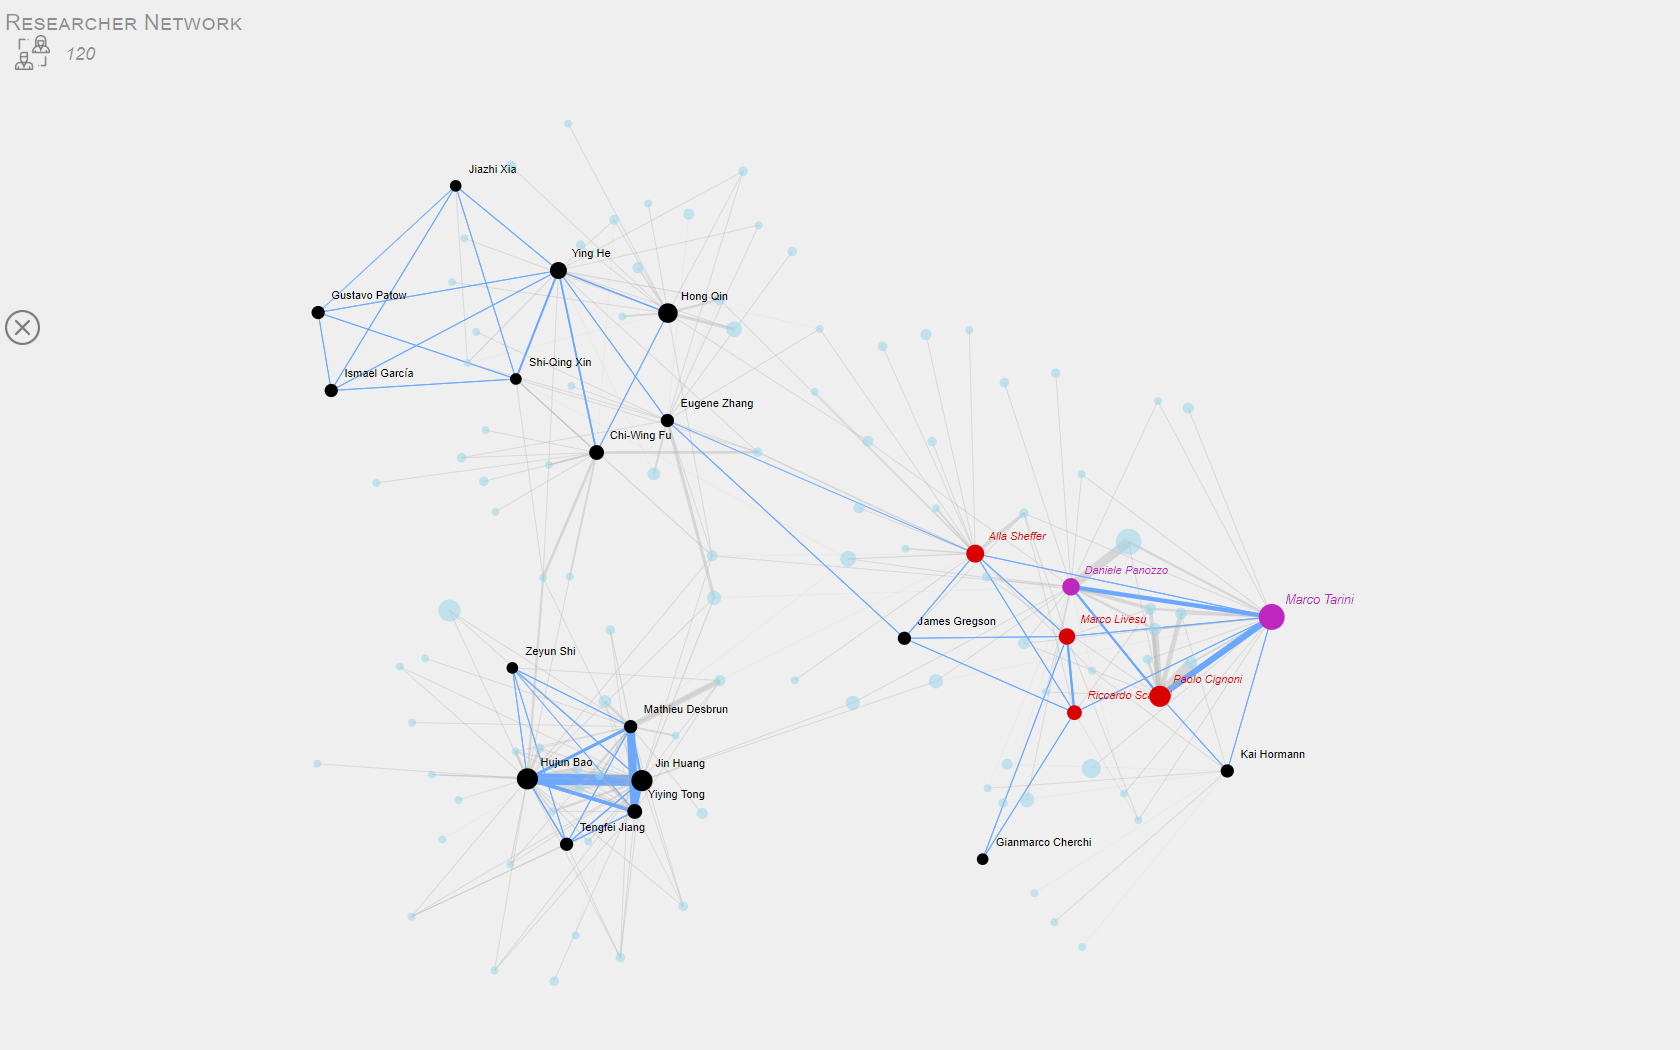
\includegraphics[width=\textwidth]{fig/researcher_network.png}
    \caption{\textcolor{red}{In the Researcher Network, arcs connect authors who have publications in common.  Arcs are blue when the co-authored papers include a selected paper. The colouring of nodes \textcolor{red}{and names} emphasizes roles as in the Researcher Timeline, while the relevance of authors is rendered through the dimension of nodes \textcolor{red}{and fonts}. The thickness of arcs renders the number of co-authored papers. The visualization can be fine-tuned by adjusting a set of parameters defining the criteria on productivity to be included in the visualization, or the criteria that define conflicts (cf. the end of this Section for their definition).}}%When hovering over an entity representing a paper, the authors of that paper are highlighted in the other views.}
    \label{fig:communities}
\end{figure*}

\textcolor{red}{Then,} the visual composition of the four regions in the interface (Figure~\ref{fig:interface}) helps the user to gain different perspectives on the problem at hand, within a single visualization. Each region can be resized in height; \textcolor{red}{the Researcher Network can be made full-screen, as in Figure \ref{fig:communities}, for better visualization and interaction.}

The nodes in the Paper Network (PN), at the bottom-left hand side of the screen, represent papers in $\mathcal{P}_{V}$, while the arcs represent in- and out-citation relations between them. \textcolor{red}{Apart from pathological cases, the network is by definition a DAG (Directed Acyclic Graph). The visualization \textcolor{red}{of the DAG is constrained along the horizontal direction, since} papers are ordered horizontally according to their publication year. While in the previous platform version \cite{stag19} a force-directed graph drawing algorithm determined the layout in the vertical direction \cite{D3js11}, in the new version we preferred a visualization which puts focus on nodes with degree higher than one, that is, on papers which cite/are cited by more than one selected paper. Those papers are are likely to represent relevant papers in the field, and therefore good candidates for being selected as key papers and expanded in the network. Therefore, each key paper is assigned a rectangular region of predefined vertical height; all its citing/cited papers with node degree equal to one are arranged inside the rectangle, whereas nodes with higher degree are positioned in-between the rectangular regions. Their positions minimize the sum of distances from the citing/cited selected papers. This visualization of the network enables one to easily detect higher-degree nodes and network cliques, and tell apart relevant papers, which are good candidates for node selection and expansion.} 

Each line in the Researcher Timeline (RT), at the upper-left side of the screen, represents a candidate reviewer $r$ in $\mathcal{R}_{C}$, that is, the author of a selected paper in $\mathcal{P}_{S}$. The dots over the line represent the set $\mathcal{P}|_{r}$ of papers authored by $r$ in the reference database $\mathcal{P}$. %The Researcher Timeline is constructed and updated automatically by ReviewerNet while the user builds and refines the Paper Network.  

The nodes in the Researcher Network (RN), at the upper-right hand side of the screen, are the researchers in $\mathcal{R}_V$ along with their collaborators in $\mathcal{R}$. The arcs connect authors who have publications in common: for each node representing a researcher $r$, the node degree is the cardinality $\vert \mathcal{CA}(r) \vert$. A force-directed graph drawing algorithm determines the graph layout, \textcolor{red}{so that authors who have a large number of publications in common tend to be close to each other}. Both the Researcher Timeline and the Researcher Network are built automatically by ReviewerNet while the user builds the Paper Network.  

The Control Panel (CP), at the bottom-right hand side of the screen, allows the user to input and manage the names of submitting authors, the names of selected reviewers, and the titles of key papers. The CP area also displays information about papers, upon request. The DBLP icon beside reviewers' names and paper titles links to their respective DBLP page. Moreover, the CP includes parameters boxes and check-boxes to fine-tune the visualization:

\noindent{\bf Size of data visualized:} 
To limit the number of candidate reviewers visualized in the RT and the RN, the user can set two thresholds a researcher has to meet to be considered as a candidate reviewer: 
\begin{itemize}
\item \emph{Productivity threshold}: the minimum number of authored selected papers in $\mathcal{P}_S$ (i.e., $\vert \mathcal{P}_{S}|_{r} \vert$ has to be greater than the threshold, for a researcher $r$ to be included in the set $\mathcal{R}_C$ of candidate reviewers);
\item \emph{Researcher expiration}: the maximum number of years since the last authored paper in the reference dataset $\mathcal{P}$ (i.e., the number of years has to be lower than the threshold for a researcher to be considered active and included in $\mathcal{R}_C$).
\end{itemize}
The user can also remove conflicting authors and their co-authors from the visualization, by ticking the \emph{Hide Conflicted} checkbox.
To augment instead the number of potential reviewers visualized, the user can tick the \emph{Expand RT \& RN} checkbox: the visualization will include all the researchers in $\mathcal{R}_V$ (all the authors of relevant papers) instead of the researchers in $\mathcal{R}_C$ only (the authors of selected papers only). Note that visualizing a large number of researchers can slow down the interface. \\

\noindent{\bf Conflict-of-interest:} 
Finally, to modulate the conflict of interest, the user can set a threshold for two researchers to be considered as co-authors, namely 
\begin{itemize}
\item \emph{Conflict expiration}: the maximum number of years since the last co-authored paper in $\mathcal{P}$. 
\end{itemize}
A larger threshold will increase the number of candidates marked as conflicted. Conversely, a smaller threshold will increase the number of available reviewers. 

\section{Visual consistency}
\label{subsec:visualvar}

Visual cues include the \textcolor{red}{position}, colour, size, boundary, and style of visual elements representing papers, researchers and their relations across the different views.  

%\noindent{\bf Visual cues for papers}
\paragraph*{Visual cues for papers} 
For a paper $p \in \mathcal{P}_{V}$, the color \textcolor{red}{may correspond either} to the citation count $c(p)$ -- from yellow (few citations) to green (many citations) -- \textcolor{red}{or to the venue where it is published -- according to the eight-value color scale in \cite{Wa13} for the most relevant venues, plus grey for the others; the relevance of a venue is given by its number of incoming citations in the dataset}. The colormap applies to both nodes in the PN and dots in the RT. Dots corresponding to papers in $\mathcal{P} - \mathcal{P}_V$ (papers in the reference database, but not included the PN) are marked as grey. 
Selected papers in $\mathcal{P}_S$ are circled in blue, both in the PN and the RT.  Arcs are blue in the RN when the co-authored papers include a selected paper.  


\begin{figure}[!t]
    \centering
    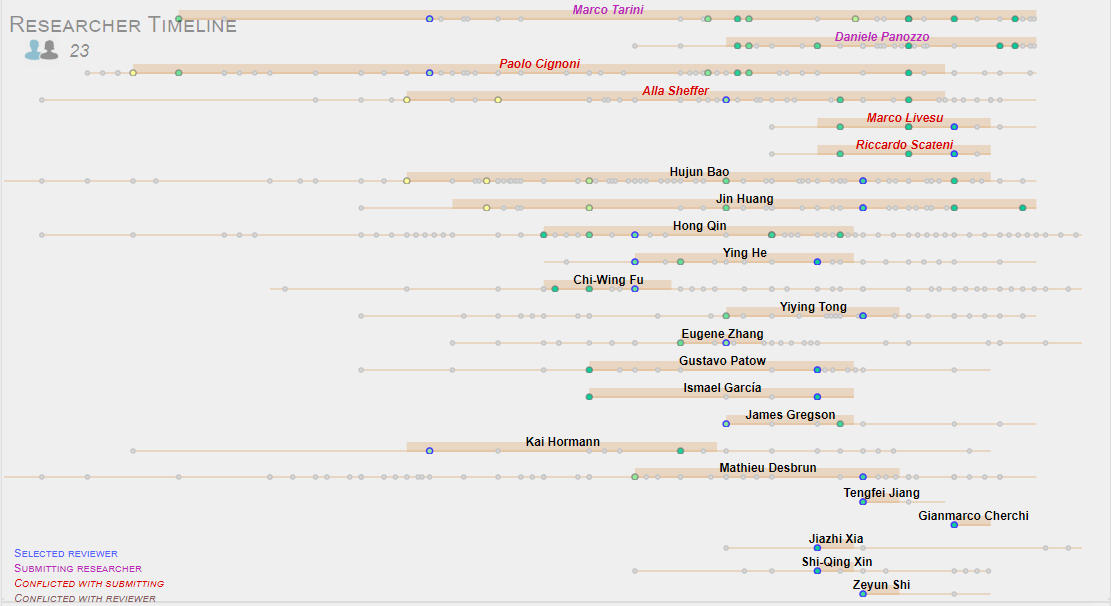
\includegraphics[width=\textwidth]{fig/timeline_cropped.png}
    \caption{\textcolor{red}{The Researcher Timeline lists the names of potential reviewers. The name colouring emphasizes the distinction among roles: submitting authors (marked as purple), their co-authors (red), selected reviewers (blue), their co-authors (brown), and non-conflicting, candidate reviewers (black). The font style of names further helps to tell apart conflicting researchers (italic) from non-conflicting candidate reviewers (normal). The \textcolor{red}{candidate reviewers} are ordered vertically according to their relevance (cf. Chapter \ref{sec:notation} for details).}}%When hovering over an entity representing a paper, the authors of that paper are highlighted in the other views.}
    \label{fig:selected}
\end{figure}


\paragraph*{Visual cues for researchers} 
For researchers in the RT, the name colouring emphasizes the distinction between roles: submitting authors (marked as purple), their co-authors (red), selected reviewers (blue), their co-authors (brown), and non-conflicting, candidate reviewers (black). The nodes in the RN corresponding to researchers in the RT follow the same rule, whereas nodes representing their co-authors in $\mathcal{R}$ are light blue \textcolor{red}{and have no name labels attached}.   
For researchers in the RT, the font style of names further helps to tell apart conflicting researchers (italic) from non-conflicting candidate reviewers (normal). The same colour/font rules apply to the names suggested in the selected reviewers' drop-down menu in the CP.
The \textcolor{red}{candidate reviewers} in the RT are ordered vertically according to their relevance score (Figure \ref{fig:selected}). The same score is rendered in the RN through the dimension of nodes.  

\section{Actions}
\label{subsec:actions}

Each view (PN, RT, RN, CP) is linked to the other views, so that any action in a view is reflected in the others. \textcolor{red}{The shortcut key $Ctrl+Z$ enables the user to undo an action.}

\begin{figure*}[!t]
    \centering
    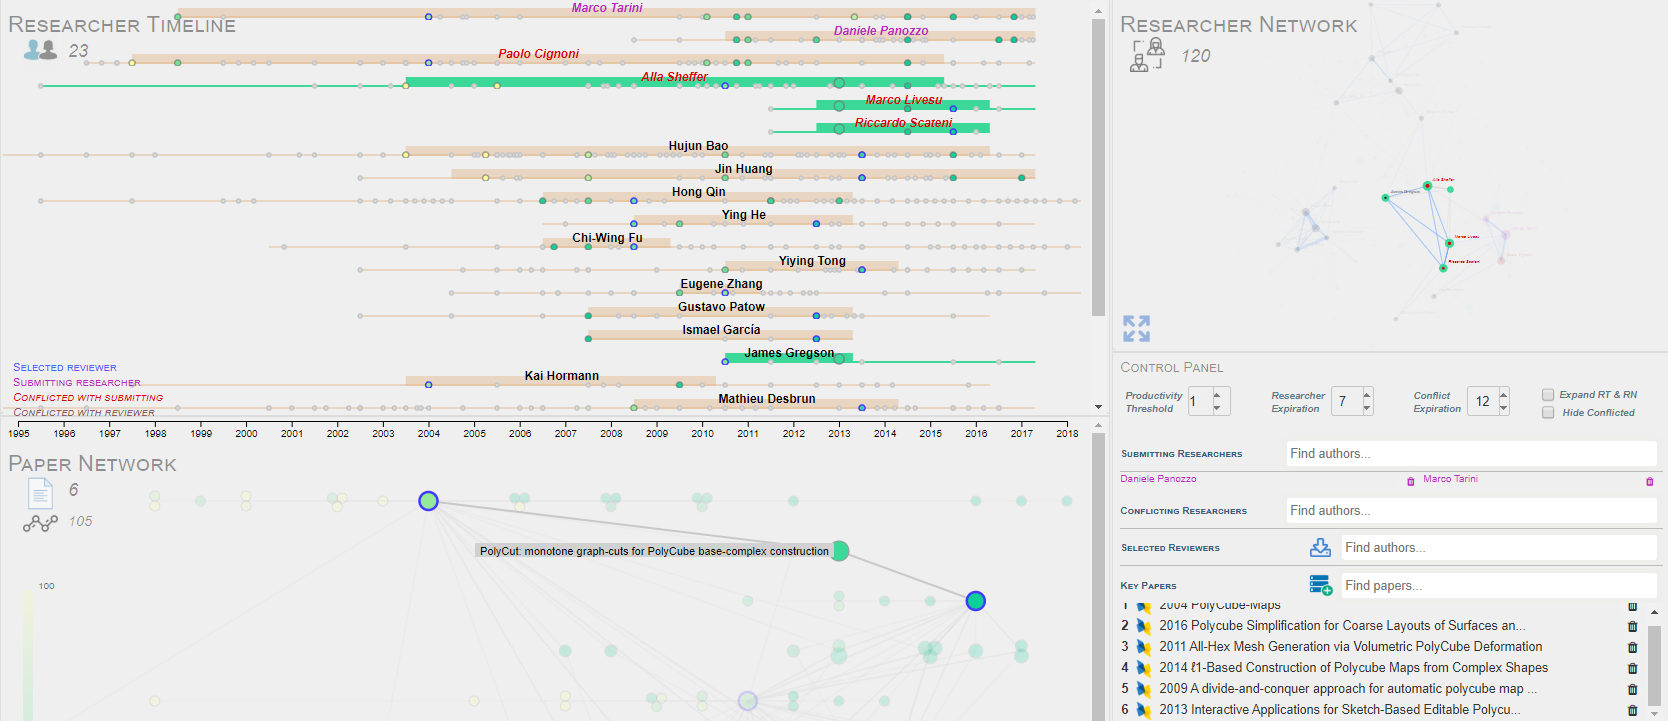
\includegraphics[width=\textwidth]{fig/timeline_paperhover.png}
    \caption{\textcolor{red}{In the Researcher Timeline, researchers are represented as horizontal lines, spanning their academic career; the bars over the lines indicate the years in which the authors published about the submission topic, namely, the years for which they have papers in the Paper Network. When hovering over an entity representing a paper, the authors of that paper are highlighted in the other views.}}
    \label{fig:overpaper}
\end{figure*}

\paragraph*{Actions on Papers} 
The user initialises the Paper Network with small set of seed papers. \textcolor{red}{The user can either type the titles of the seed papers} in the \emph{Key papers} field, with the help of title-based suggestions, \textcolor{red}{or press the \emph{Import from bibliography} button and paste a list of references. The references are parsed to identify matching titles in the dataset through a fuzzy search; the candidate titles with higher scores are shown to the user, who can select or discard them. Then,} the seed papers are visualized in the PN, along with their in- and out-citations. The user can now expand the network, to discover additional documents. With a double click, he selects interesting nodes, i.e., papers he/she deems relevant to the submission topic. The PN then updates with the in- and out-citations of the selected papers. 

Papers can be deselected \textcolor{red}{either with a double click or through the trash bin icon in the Control Panel}. 

When the users focuses on a paper in one of the views by mouse hovering, the same paper is highlighted in the other views. For example, when hovering the mouse over a node in the PN, the corresponding dot in the Researcher Timeline is highlighted, and vice-versa. Also, the paper details (title, publication year, venue) are shown in the Control Panel on a mouse click. Likewise, by hovering over or clicking on the title in the CP, the corresponding node and dot are highlighted in the PN and the RT. When hovering the mouse over an entity representing a paper (a node in the PN, a dot in the RT bars, the title in the CP), the paper authors are highlighted in the RT and RN, if present (Figure \ref{fig:overpaper}). A mouse click on the focused paper lets the user navigate the visualization with highlighted items. A single click restores the previous visualization.
The icon beside paper titles in the Control Panel links to DBLP pages. 

\paragraph*{Actions on Researchers} In a similar fashion to papers, when the user focuses on a researcher in one of the views by mouse hovering, the same researcher is highlighted in the other views. When hovering the mouse over a node in the Researcher Network, the name of the corresponding researcher appears on the upper-right corner.  
When hovering the mouse over an entity representing a researcher (a bar in the RT, a dot in the RN, the name in the CP), the papers authored by the researcher are highlighted in the Paper Network view. 
In Figure \ref{fig:authorclick}, a mouse click on a researcher puts the focus on him/her, his/her production and his/her personal net of collaborators. 

\begin{figure}[!ht]
    \centering
    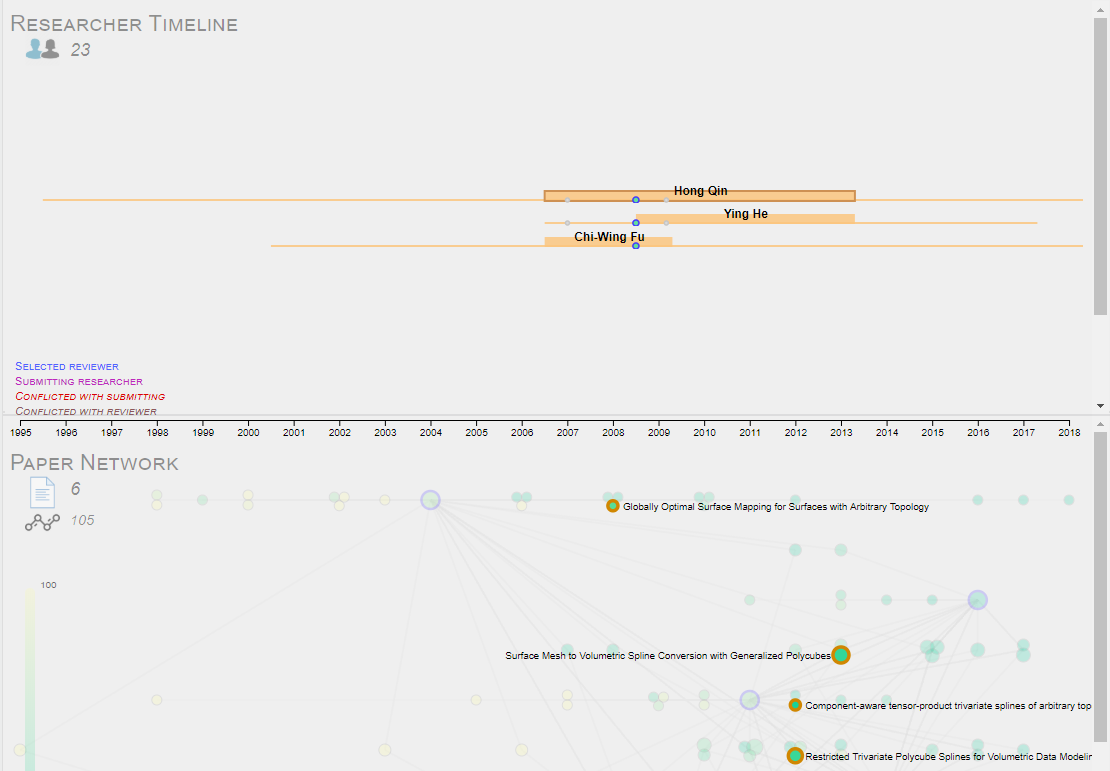
\includegraphics[width=0.8\textwidth, height=6cm]{fig/timeline_researcherhover_cropped.png}
    \caption{\textcolor{red}{Focusing on a researcher by clicking on her/his name in the Researcher Timeline allows one to highlight her/his co-authors and production in the Paper Network.}}%When hovering over an entity representing a paper, the authors of that paper are highlighted in the other views.}
    \label{fig:authorclick}
\end{figure}

The user can navigate a visualization with selected items and additional functionalities. Only the set of co-authors is visualized in the Researcher Timeline and the Researcher Network. While hovering on one of the co-authors, the common publications are shown in the PN, and the arc representing the co-authorship relation is visualized in the RN. Another mouse click will get the user back the previous visualization.
When hovering the mouse over an arc in the RT, like in Figure \ref{fig:researchernetwork}, a pop-up on the upper-right corner shows the pair of co-authors names, the number of common papers in the dataset $\mathcal{P}$, and the number of common relevant papers in $\mathcal{P}_{V}$. In turn, for blue arcs, the common papers are highlighted in the PN. 

\begin{figure*}[!ht]
    \centering
    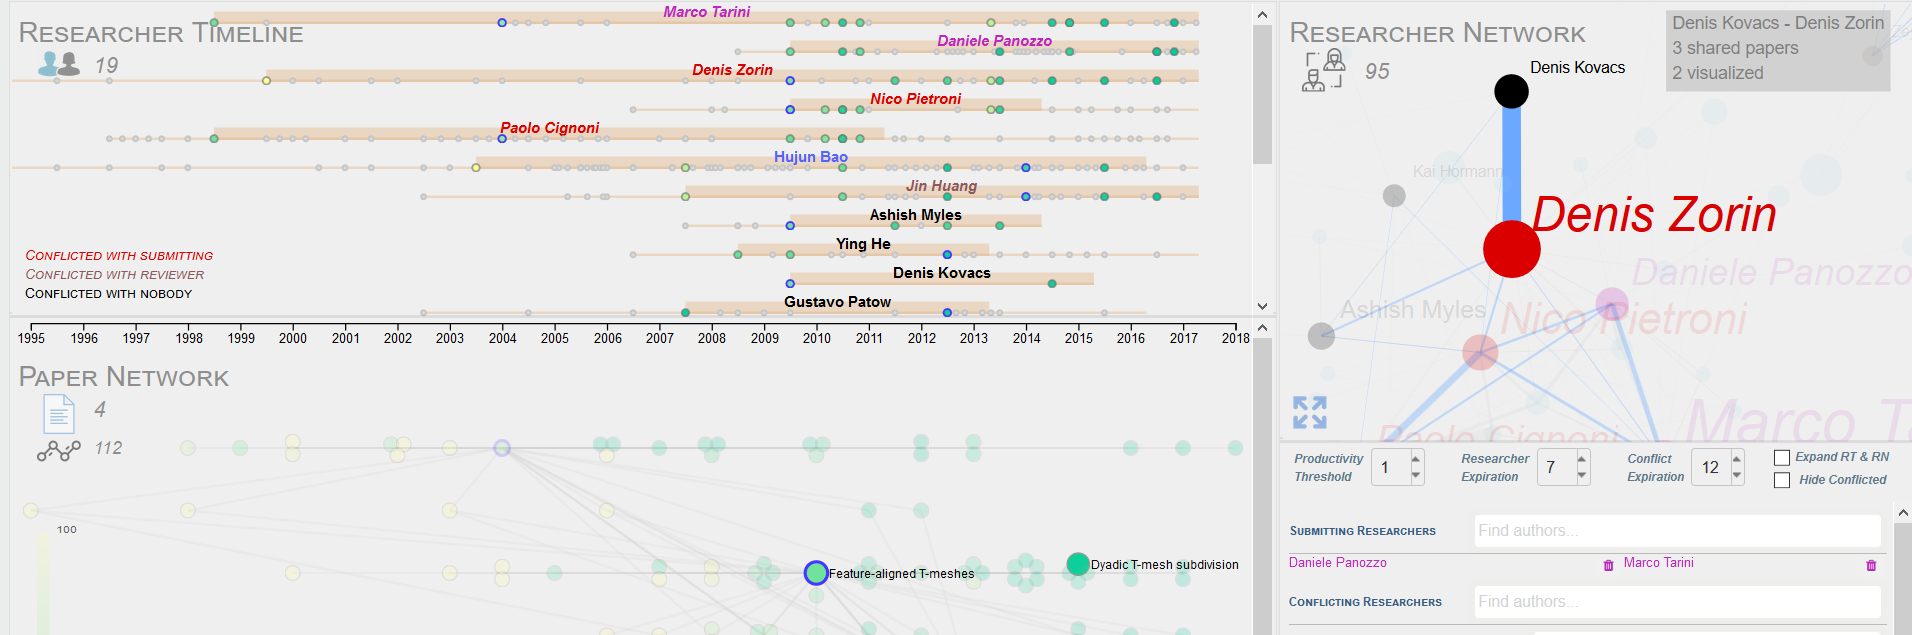
\includegraphics[width=\textwidth]{fig/researchernetwork.png}
    \caption{Hovering over a segment joining two researchers in the Researcher Network shows details about their co-authored papers and highlights them in the Paper Network.}
    \label{fig:researchernetwork}
    \end{figure*}

The icon beside the researcher name in any of the fields in the Control Panel links to the DBLP page of that researcher. 
A researcher can be removed from the list of selected reviewers \textcolor{red}{either with a double click or through the trash bin icon in the Control Panel}. The user can exchange a reviewer with one of his/her substitutes by clicking on the name of the substitute.
The export button enables the user to download the list of reviewers and their potential substitutes. Work sessions can be saved for later re-use and re-assessment. 